% !TEX root = ../../thesis.tex
% \newpage
\section{Adding novel mechanisms to Poppy} % (fold)
\label{sec:morphology-add-mechanism}

\textbf{context:} Poppy has been made to allow quick and cheap exploration and experimentation of morphological variation (i.e. change of its hardware).
\textbf{need:}
We are interested in the design of increasingly under-actuated robots. We especially want to explore semi-passive ability and use of natural body properties rather than using actuation power to achieve dynamic tasks. Until now,  humanoid bipedal locomotion has mostly been achieved using ZMP control leading to walking gait with the knees always bended. The permanent high torque and foot impacts applied to the knee require high-powered actuators.
\textbf{Task:} With Poppy, we wanted to explore a mechanical design that reduces the required power. We decided to test the use of a semi-passive knee joint based on a MX-28 Dynamixel motor completed with a parallel spring system.
\textbf{objet:} We will explain how we create this mechanism by changing the mechanical design of Poppy's legs and we will present the results we obtained during walking experiments.

We explore the design of a semi-passive mechanism with the aim of assisting the motor during two critical phases of the walking gait:
\begin{enumerate}
    \item the foot impact, which can produce an abrupt raise of load in the knee during stance phase,
    \item the flexion of the leg during swing phase.
\end{enumerate}

\subsection{Semi-passive knee mechanism principle} % (fold)
For this purpose we chose a mechanism inspired by that of Gini and Scarfogliero~\parencite{gini2009new} involving two traction springs positioned in parallel to the knee joint in such a way that there are two low-potential solutions, one when the leg is straight and one when the leg is bended (see \figurename~\ref{fig:Gini_knee}).

\begin{figure}[]
\centering
    \subfloat[][Actual design of the robot knee.]{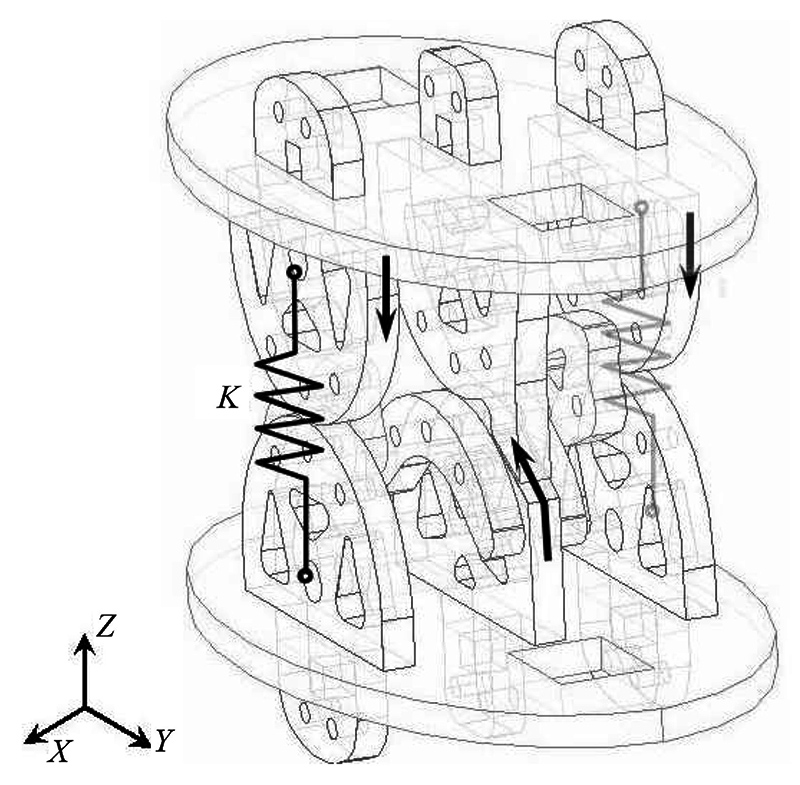
\includegraphics[height=5cm]{Gini_knee_design.jpg}}
    \hfil
    \subfloat[][Mechanism principle.]{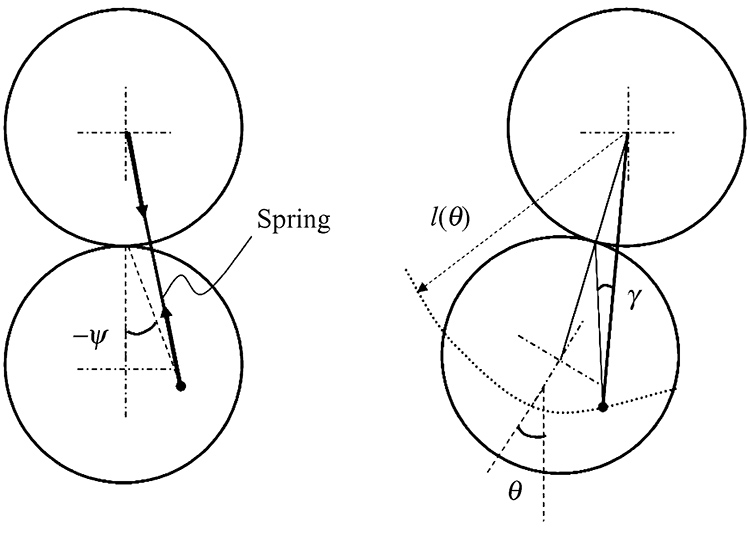
\includegraphics[height=5cm]{Gini_knee_mechanism.jpg}}
    \caption{Gini and Scarfogliero designed a bio-inspired knee joint which uses parallel traction springs to both bend the leg and keep it straight. Illustrations extracted from~\parencite{gini2009new}.}
    \label{fig:Gini_knee}
\end{figure}

Therefore this mechanism can participate in the leg dynamic and assist the motor during two walking main phases:
\begin{itemize}
    \item They help to keep the leg straight during the support phase without any motor control.
    \item During the swing phase, they participate in the flexion of the leg.
\end{itemize}

These two modes can be passively switched by the actual knee angle, yet we have to determine which angle is the most suitable. Considering the human knee kinematic (see Fig.~\ref{fig:human_knee_kinematic}), we chose to change mode at $\theta_{knee} = 20+5$\textsuperscript{o}  which corresponds to a transition between the stance preparation phase and the swing phase.

\begin{figure}[thpb]
    \centering
    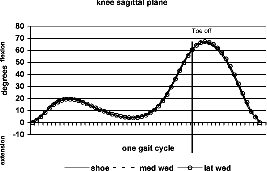
\includegraphics[width=0.6\linewidth]{knee_kinematic.pdf}
    \caption{Actual flexion kinematic of a human knee during the walking gait~\parencite{Nester2003}. We can identify two main phases corresponding to the stance preparation phase and the swing phase. The main difference is the amplitude of the motion i.e $<20$\textsuperscript{o}  for the stance phase and $>20$\textsuperscript{o} for the swing phase.}
    \label{fig:human_knee_kinematic}
\end{figure}


\subsection{Experimentation on Poppy} % (fold)

An illustration of the real behavior is shown in the videos \url{https://vimeo.com/63839782}

\begin{figure}[ht]
    \begin{center}
        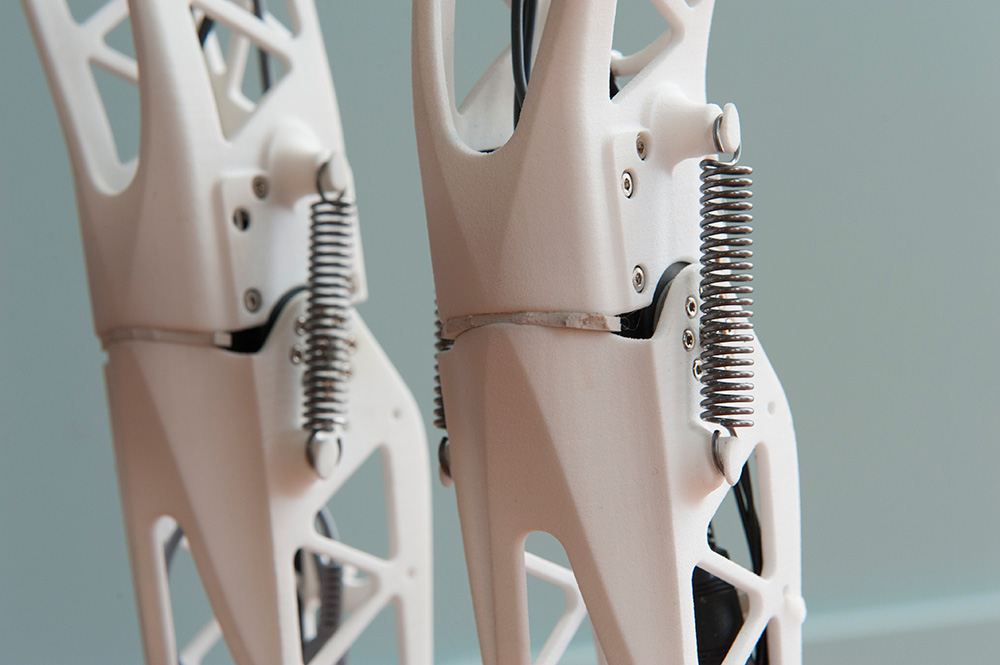
\includegraphics[width=0.6\linewidth]{poppy_semi_passive_knee.jpg}
    \end{center}
    \caption{}

\end{figure}


\begin{figure}[!ht]
\centering
    \subfloat[][without springs]{\label{fig:knee_wout_spring}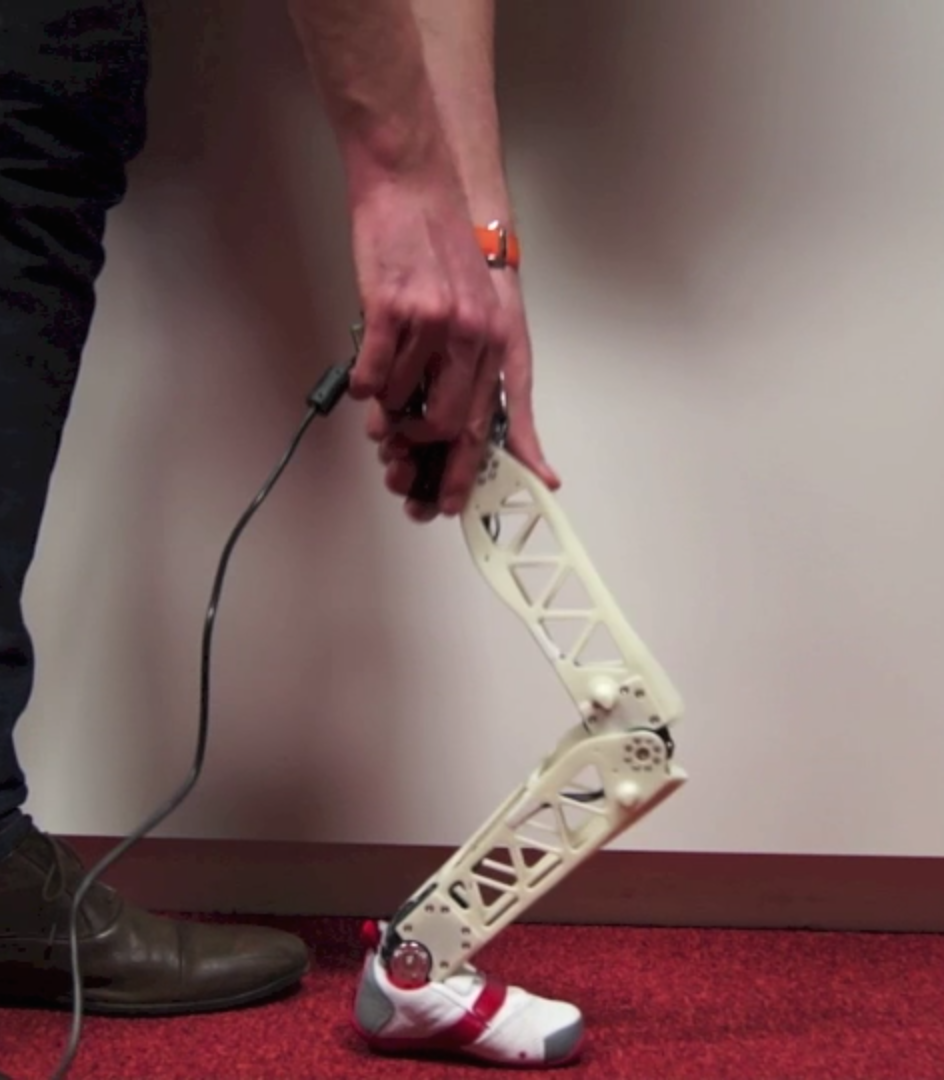
\includegraphics[height=6cm]{knee_wout_spring.png}}
    \hfil
    \subfloat[][with traction spring]{\label{fig:knee_w_spring}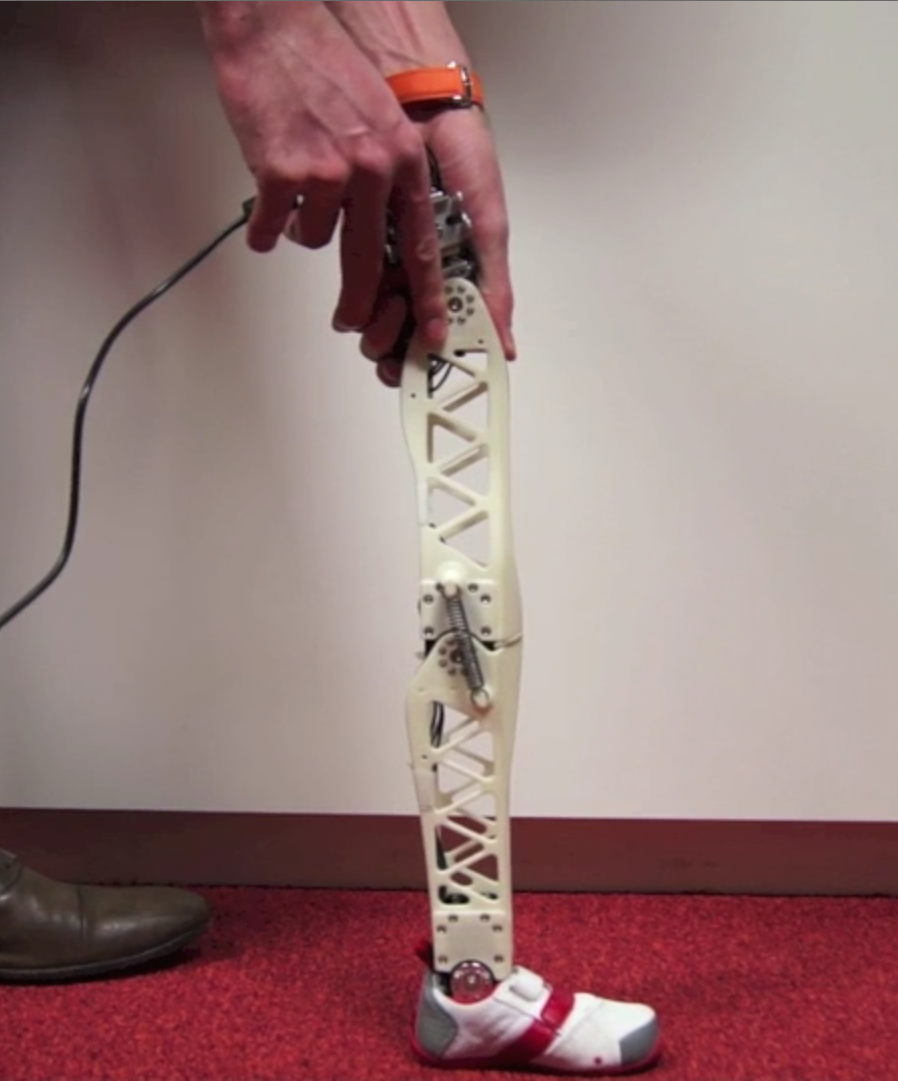
\includegraphics[height=6cm]{knee_w_spring}}
    \caption{Motors fully compliant \url{https://vimeo.com/63839782}}

\end{figure}




